\section{Simulation Settings}

\color{RoyalPurple}\begin{verbatim}
simulation.numb_odes = 100;          % number of ODEs
% observation noise
simulation.state_obs_variance = @(mean)(bsxfun(@times,0.1,ones(size(mean))));
simulation.ode_param = 8;            % true ODE parameter;
simulation.final_time = 4;           % end time for integration
simulation.int_interval = 0.01;      % integration interval
simulation.time_samp = 0:0.125:simulation.final_time; % sample times for observations
simulation.init_val = zeros(1,simulation.numb_odes); % initial state values

% ratio of number of observed states over number of unobserved states.
simulation.observed_states = 0.5;    % only 50% of the states are observed
\end{verbatim}
\color{black}


\section{User Input}

\begin{par}
\subsection{ Path to ODEs }
\end{par} \vspace{1em}
\color{RoyalPurple}\begin{verbatim}
odes_path = 'Lorenz96_ODEs.txt';
\end{verbatim}
\color{black}
\begin{par}
\subsection{ Symbols } symbols of states and parameters in the '\_ODEs.txt' file
\end{par} \vspace{1em}
\begin{par}
States $\mathbf{x}$:
\end{par} \vspace{1em}
\color{RoyalPurple}\begin{verbatim}
for u = 1:simulation.numb_odes; symbols.state(u) = {['[x_' num2str(u) ']']}; end
\end{verbatim}
\color{black}
\begin{par}
ODE parameters $\theta$ (symbols of parameters in 'ODEs.txt' file):
\end{par} \vspace{1em}
\color{RoyalPurple}\begin{verbatim}
symbols.param = {'[\theta]'};
% \section{ Kernel }
%
% Kernel parameters $\phi$:
kernel.param = [10,0.2];             % set values of rbf kernel parameters
\end{verbatim}
\color{black}
\begin{par}
Error variance on state derivatives (i.e. $\gamma$):
\end{par} \vspace{1em}
\color{RoyalPurple}\begin{verbatim}
state.derivative_variance = 6*ones(1,length(symbols.state)); % gamma for gradient matching model
\end{verbatim}
\color{black}
\begin{par}
\subsection{ Estimation times }
\end{par} \vspace{1em}
\color{RoyalPurple}\begin{verbatim}
time.est = 0:0.1:4;                 % estimation times
\end{verbatim}
\color{black}
\begin{par}
\subsection{ Type of pseudo-inverse } Type of pseudo inverse; options: 'Moore-Penrose' or 'modified Moore-Penrose'
\end{par} \vspace{1em}
\color{RoyalPurple}\begin{verbatim}
opt_settings.pseudo_inv_type = 'Moore-Penrose';
\end{verbatim}
\color{black}
\begin{par}
\subsection{ Optimization settings }
\end{par} \vspace{1em}
\color{RoyalPurple}\begin{verbatim}
opt_settings.coord_ascent_numb_iter = 10;  % number of coordinate ascent iterations

% The observed state trajectories are clamped to the trajectories
% determined by standard GP regression (Boolean)
opt_settings.clamp_obs_state_to_GP_fit = true;
\end{verbatim}
\color{black}
\begin{par}
Plot settings: layout and size
\end{par} \vspace{1em}
\color{RoyalPurple}\begin{verbatim}
plot_settings.size = [1600, 800]; plot_settings.layout = [3,3];
\end{verbatim}
\color{black}


\section{Import ODEs}

\color{RoyalPurple}\begin{verbatim}
generate_Lorenz96_ODEs(simulation.numb_odes)
ode = import_odes(symbols,odes_path);
\end{verbatim}
\color{black}
\color{RoyalPurple}\begin{verbatim}
disp('ODEs:'); disp(ode.raw)
\end{verbatim}
\color{black}

        \begin{verbatim}ODEs:
    '([x_2] - [x_99]) .* [x_100] - [x_1] + [\theta]'
    '([x_3] - [x_100]) .* [x_1] - [x_2] + [\theta]'
    '([x_4] - [x_1]) .* [x_2] - [x_3] + [\theta]'
    '([x_5] - [x_2]) .* [x_3] - [x_4] + [\theta]'
    '([x_6] - [x_3]) .* [x_4] - [x_5] + [\theta]'
    '([x_7] - [x_4]) .* [x_5] - [x_6] + [\theta]'
    '([x_8] - [x_5]) .* [x_6] - [x_7] + [\theta]'
    '([x_9] - [x_6]) .* [x_7] - [x_8] + [\theta]'
    '([x_10] - [x_7]) .* [x_8] - [x_9] + [\theta]'
    '([x_11] - [x_8]) .* [x_9] - [x_10] + [\theta]'
    '([x_12] - [x_9]) .* [x_10] - [x_11] + [\theta]'
    '([x_13] - [x_10]) .* [x_11] - [x_12] + [\theta]'
    '([x_14] - [x_11]) .* [x_12] - [x_13] + [\theta]'
    '([x_15] - [x_12]) .* [x_13] - [x_14] + [\theta]'
    '([x_16] - [x_13]) .* [x_14] - [x_15] + [\theta]'
    '([x_17] - [x_14]) .* [x_15] - [x_16] + [\theta]'
    '([x_18] - [x_15]) .* [x_16] - [x_17] + [\theta]'
    '([x_19] - [x_16]) .* [x_17] - [x_18] + [\theta]'
    '([x_20] - [x_17]) .* [x_18] - [x_19] + [\theta]'
    '([x_21] - [x_18]) .* [x_19] - [x_20] + [\theta]'
    '([x_22] - [x_19]) .* [x_20] - [x_21] + [\theta]'
    '([x_23] - [x_20]) .* [x_21] - [x_22] + [\theta]'
    '([x_24] - [x_21]) .* [x_22] - [x_23] + [\theta]'
    '([x_25] - [x_22]) .* [x_23] - [x_24] + [\theta]'
    '([x_26] - [x_23]) .* [x_24] - [x_25] + [\theta]'
    '([x_27] - [x_24]) .* [x_25] - [x_26] + [\theta]'
    '([x_28] - [x_25]) .* [x_26] - [x_27] + [\theta]'
    '([x_29] - [x_26]) .* [x_27] - [x_28] + [\theta]'
    '([x_30] - [x_27]) .* [x_28] - [x_29] + [\theta]'
    '([x_31] - [x_28]) .* [x_29] - [x_30] + [\theta]'
    '([x_32] - [x_29]) .* [x_30] - [x_31] + [\theta]'
    '([x_33] - [x_30]) .* [x_31] - [x_32] + [\theta]'
    '([x_34] - [x_31]) .* [x_32] - [x_33] + [\theta]'
    '([x_35] - [x_32]) .* [x_33] - [x_34] + [\theta]'
    '([x_36] - [x_33]) .* [x_34] - [x_35] + [\theta]'
    '([x_37] - [x_34]) .* [x_35] - [x_36] + [\theta]'
    '([x_38] - [x_35]) .* [x_36] - [x_37] + [\theta]'
    '([x_39] - [x_36]) .* [x_37] - [x_38] + [\theta]'
    '([x_40] - [x_37]) .* [x_38] - [x_39] + [\theta]'
    '([x_41] - [x_38]) .* [x_39] - [x_40] + [\theta]'
    '([x_42] - [x_39]) .* [x_40] - [x_41] + [\theta]'
    '([x_43] - [x_40]) .* [x_41] - [x_42] + [\theta]'
    '([x_44] - [x_41]) .* [x_42] - [x_43] + [\theta]'
    '([x_45] - [x_42]) .* [x_43] - [x_44] + [\theta]'
    '([x_46] - [x_43]) .* [x_44] - [x_45] + [\theta]'
    '([x_47] - [x_44]) .* [x_45] - [x_46] + [\theta]'
    '([x_48] - [x_45]) .* [x_46] - [x_47] + [\theta]'
    '([x_49] - [x_46]) .* [x_47] - [x_48] + [\theta]'
    '([x_50] - [x_47]) .* [x_48] - [x_49] + [\theta]'
    '([x_51] - [x_48]) .* [x_49] - [x_50] + [\theta]'
    '([x_52] - [x_49]) .* [x_50] - [x_51] + [\theta]'
    '([x_53] - [x_50]) .* [x_51] - [x_52] + [\theta]'
    '([x_54] - [x_51]) .* [x_52] - [x_53] + [\theta]'
    '([x_55] - [x_52]) .* [x_53] - [x_54] + [\theta]'
    '([x_56] - [x_53]) .* [x_54] - [x_55] + [\theta]'
    '([x_57] - [x_54]) .* [x_55] - [x_56] + [\theta]'
    '([x_58] - [x_55]) .* [x_56] - [x_57] + [\theta]'
    '([x_59] - [x_56]) .* [x_57] - [x_58] + [\theta]'
    '([x_60] - [x_57]) .* [x_58] - [x_59] + [\theta]'
    '([x_61] - [x_58]) .* [x_59] - [x_60] + [\theta]'
    '([x_62] - [x_59]) .* [x_60] - [x_61] + [\theta]'
    '([x_63] - [x_60]) .* [x_61] - [x_62] + [\theta]'
    '([x_64] - [x_61]) .* [x_62] - [x_63] + [\theta]'
    '([x_65] - [x_62]) .* [x_63] - [x_64] + [\theta]'
    '([x_66] - [x_63]) .* [x_64] - [x_65] + [\theta]'
    '([x_67] - [x_64]) .* [x_65] - [x_66] + [\theta]'
    '([x_68] - [x_65]) .* [x_66] - [x_67] + [\theta]'
    '([x_69] - [x_66]) .* [x_67] - [x_68] + [\theta]'
    '([x_70] - [x_67]) .* [x_68] - [x_69] + [\theta]'
    '([x_71] - [x_68]) .* [x_69] - [x_70] + [\theta]'
    '([x_72] - [x_69]) .* [x_70] - [x_71] + [\theta]'
    '([x_73] - [x_70]) .* [x_71] - [x_72] + [\theta]'
    '([x_74] - [x_71]) .* [x_72] - [x_73] + [\theta]'
    '([x_75] - [x_72]) .* [x_73] - [x_74] + [\theta]'
    '([x_76] - [x_73]) .* [x_74] - [x_75] + [\theta]'
    '([x_77] - [x_74]) .* [x_75] - [x_76] + [\theta]'
    '([x_78] - [x_75]) .* [x_76] - [x_77] + [\theta]'
    '([x_79] - [x_76]) .* [x_77] - [x_78] + [\theta]'
    '([x_80] - [x_77]) .* [x_78] - [x_79] + [\theta]'
    '([x_81] - [x_78]) .* [x_79] - [x_80] + [\theta]'
    '([x_82] - [x_79]) .* [x_80] - [x_81] + [\theta]'
    '([x_83] - [x_80]) .* [x_81] - [x_82] + [\theta]'
    '([x_84] - [x_81]) .* [x_82] - [x_83] + [\theta]'
    '([x_85] - [x_82]) .* [x_83] - [x_84] + [\theta]'
    '([x_86] - [x_83]) .* [x_84] - [x_85] + [\theta]'
    '([x_87] - [x_84]) .* [x_85] - [x_86] + [\theta]'
    '([x_88] - [x_85]) .* [x_86] - [x_87] + [\theta]'
    '([x_89] - [x_86]) .* [x_87] - [x_88] + [\theta]'
    '([x_90] - [x_87]) .* [x_88] - [x_89] + [\theta]'
    '([x_91] - [x_88]) .* [x_89] - [x_90] + [\theta]'
    '([x_92] - [x_89]) .* [x_90] - [x_91] + [\theta]'
    '([x_93] - [x_90]) .* [x_91] - [x_92] + [\theta]'
    '([x_94] - [x_91]) .* [x_92] - [x_93] + [\theta]'
    '([x_95] - [x_92]) .* [x_93] - [x_94] + [\theta]'
    '([x_96] - [x_93]) .* [x_94] - [x_95] + [\theta]'
    '([x_97] - [x_94]) .* [x_95] - [x_96] + [\theta]'
    '([x_98] - [x_95]) .* [x_96] - [x_97] + [\theta]'
    '([x_99] - [x_96]) .* [x_97] - [x_98] + [\theta]'
    '([x_100] - [x_97]) .* [x_98] - [x_99] + [\theta]'
    '([x_1] - [x_98]) .* [x_99] - [x_100] + [\theta]'

\end{verbatim}
\color{black}
    

\section{Simulate Trajectory Observations}

\begin{par}
\subsection{ Generate ground truth by numerical integration }
\end{par} \vspace{1em}
\color{RoyalPurple}\begin{verbatim}
[state,time,ode] = generate_ground_truth(time,state,ode,symbols,simulation,...
    odes_path);
\end{verbatim}
\color{black}
\begin{par}
\subsection{ Generate state observations }
\end{par} \vspace{1em}
\color{RoyalPurple}\begin{verbatim}
if ~iscell(simulation.observed_states)
    ratio_observed = simulation.observed_states;
    state_obs_idx = zeros(1,simulation.numb_odes,'logical');
    idx = randperm(simulation.numb_odes);
    idx = idx(1:floor(simulation.numb_odes * ratio_observed));
    state_obs_idx(idx) = 1;
    simulation.observed_states = symbols.state(state_obs_idx);
end

[state,time,obs_to_state_relation] = generate_state_obs(state,time,simulation,...
    symbols);
\end{verbatim}
\color{black}
\begin{par}
\subsection{ Symbols }
\end{par} \vspace{1em}
\color{RoyalPurple}\begin{verbatim}
state.sym.mean = sym('x%d%d',[length(time.est),length(ode.system)]);
state.sym.variance = sym('sigma%d%d',[length(time.est),length(ode.system)]);
ode_param.sym.mean = sym('param%d',[length(symbols.param),1]);
assume(ode_param.sym.mean,'real');
\end{verbatim}
\color{black}
\begin{par}
\subsection{ Setup plots }
\end{par} \vspace{1em}
\begin{par}
Only the state dynamics are (partially) observed.
\end{par} \vspace{1em}
\color{RoyalPurple}\begin{verbatim}
[h_states,h_param,p] = setup_plots(state,time,simulation,symbols,plot_settings);

tic; %start timer
\end{verbatim}
\color{black}

\color{RoyalPurple}\begin{verbatim}
[dC_times_invC,inv_C,A_plus_gamma_inv] = kernel_function(kernel,state,time.est);
\end{verbatim}
\color{black}


\section{State Couplings in ODEs}

\color{RoyalPurple}\begin{verbatim}
coupling_idx = find_state_couplings_in_odes(ode,symbols);
\end{verbatim}
\color{black}

\section{Prior over State and State Derivatives}
\color{RoyalPurple}\begin{verbatim}
[dC_times_invC,inv_C,A_plus_gamma_inv] = kernel_function(kernel,state,time.est);
\end{verbatim}
\color{black}

\section{Rewrite ODEs as Linear Combination in Parameters}

\begin{par}
We rewrite the ODEs in equation (2) as a linear combination in the parameters:
\end{par} \vspace{1em}
\begin{par}
$\mathbf{B}_{\theta k} \theta + \mathbf{b}_{\theta k} \stackrel{!}{=} \mathbf{f}_k(\mathbf{X},\theta) \qquad (5)$,
\end{par} \vspace{1em}
\begin{par}
where matrices $\mathbf{B}_{\theta k}$ and $\mathbf{b}_{\theta k}$ are defined such that the ODEs $\mathbf{f}_k(\mathbf{X},\theta)$ are expressed as a linear combination in $\theta$.
\end{par} \vspace{1em}
\color{RoyalPurple}\begin{verbatim}
[ode_param.lin_comb.B,ode_param.lin_comb.b] = ...
    rewrite_odes_as_linear_combination_in_parameters(ode,symbols);
\end{verbatim}
\color{black}


\section{Rewrite ODEs as Linear Combination in Individual States}

\begin{par}
We rewrite the expression $\mathbf{f}(\mathbf{X},\theta) - {'\mathbf{C}}_{\phi} \mathbf{C}_{\phi}^{-1} \mathbf{X}$ in equation (4) as a linear combination in the individual state $\mathbf{x}_u$:
\end{par} \vspace{1em}
\begin{par}
$\mathbf{R}_{uk} \mathbf{x}_u + \mathbf{r}_{uk} \stackrel{!}{=} \mathbf{f}_k(\mathbf{X},\theta)$.
\end{par} \vspace{1em}
\begin{par}
where matrices $\mathbf{R}_{uk}$ and $\mathbf{r}_{uk}$ are defined such that the ODE $\mathbf{f}_k(\mathbf{X},\theta)$ is expressed as a linear combination in the individual state $\mathbf{x}_u$.
\end{par} \vspace{1em}
\color{RoyalPurple}\begin{verbatim}
[state.lin_comb.R,state.lin_comb.r] = ...
    rewrite_odes_as_linear_combination_in_ind_states(ode,symbols,coupling_idx.states);
\end{verbatim}
\color{black}

\section{Fitting observations of state trajectories}

\begin{par}
\color{RoyalPurple}\begin{verbatim}
[mu,inv_sigma] = fitting_state_observations(state,inv_C,obs_to_state_relation,simulation);
\end{verbatim}
\color{black}
\end{par}

\section{Coordinate Ascent Variational Gradient Matching}

\begin{par}
We minimize the KL-divergence in equation (10) by coordinate descent (where each step is analytically tractable) by iterating between determining the proxy for the distribution over ODE parameters $\hat{q}(\theta)$ and the proxies for the distribution over individual states $\hat{q}(\mathbf{x}_u)$.
\end{par} \vspace{1em}
\color{RoyalPurple}\begin{verbatim}
state.proxy.mean = mu;  % Initialize the state estimation by the GP regression posterior
for i = 1:opt_settings.coord_ascent_numb_iter
\end{verbatim}
\color{black}

\subsection{ Proxy for ODE parameters }
\color{RoyalPurple}\begin{verbatim}
    [param_proxy_mean,param_proxy_inv_cov] = proxy_for_ode_parameters(state.proxy.mean,...
        dC_times_invC,ode_param.lin_comb,symbols,A_plus_gamma_inv,opt_settings);

    if i==1 || ~mod(i,1)
        plot_results(h_states,h_param,state,time,simulation,param_proxy_mean,...
            p,symbols,'not_final');
    end
\end{verbatim}
\color{black}

\subsection{Proxy for individual states}
\color{RoyalPurple}\begin{verbatim}
    [state.proxy.mean,state.proxy.inv_cov] = proxy_for_ind_states(state.lin_comb,...
        state.proxy.mean,param_proxy_mean',dC_times_invC,coupling_idx.states,symbols,...
        mu,inv_sigma,simulation.observed_states,A_plus_gamma_inv,opt_settings);
\end{verbatim}

{
\centering
\includegraphics [width=5in]{Lorenz96_2_05.eps}

\includegraphics [width=5in]{Lorenz96_2_06.eps}

\includegraphics [width=5in]{Lorenz96_2_07.eps}

\includegraphics [width=5in]{Lorenz96_2_08.eps}

\includegraphics [width=5in]{Lorenz96_2_09.eps}

\includegraphics [width=5in]{Lorenz96_2_10.eps}

\includegraphics [width=5in]{Lorenz96_2_11.eps}

\includegraphics [width=5in]{Lorenz96_2_12.eps}

\includegraphics [width=5in]{Lorenz96_2_13.eps}

\includegraphics [width=5in]{Lorenz96_2_14.eps}
}

\color{black}
\color{RoyalPurple}\begin{verbatim}
end
\end{verbatim}
\color{black}
\begin{par}
\subsection{ Final result }
\end{par} \vspace{1em}
\color{RoyalPurple}\begin{verbatim}
plot_results(h_states,h_param,state,time,simulation,param_proxy_mean,p,symbols,'final');
\end{verbatim}
\color{black}

{
\centering
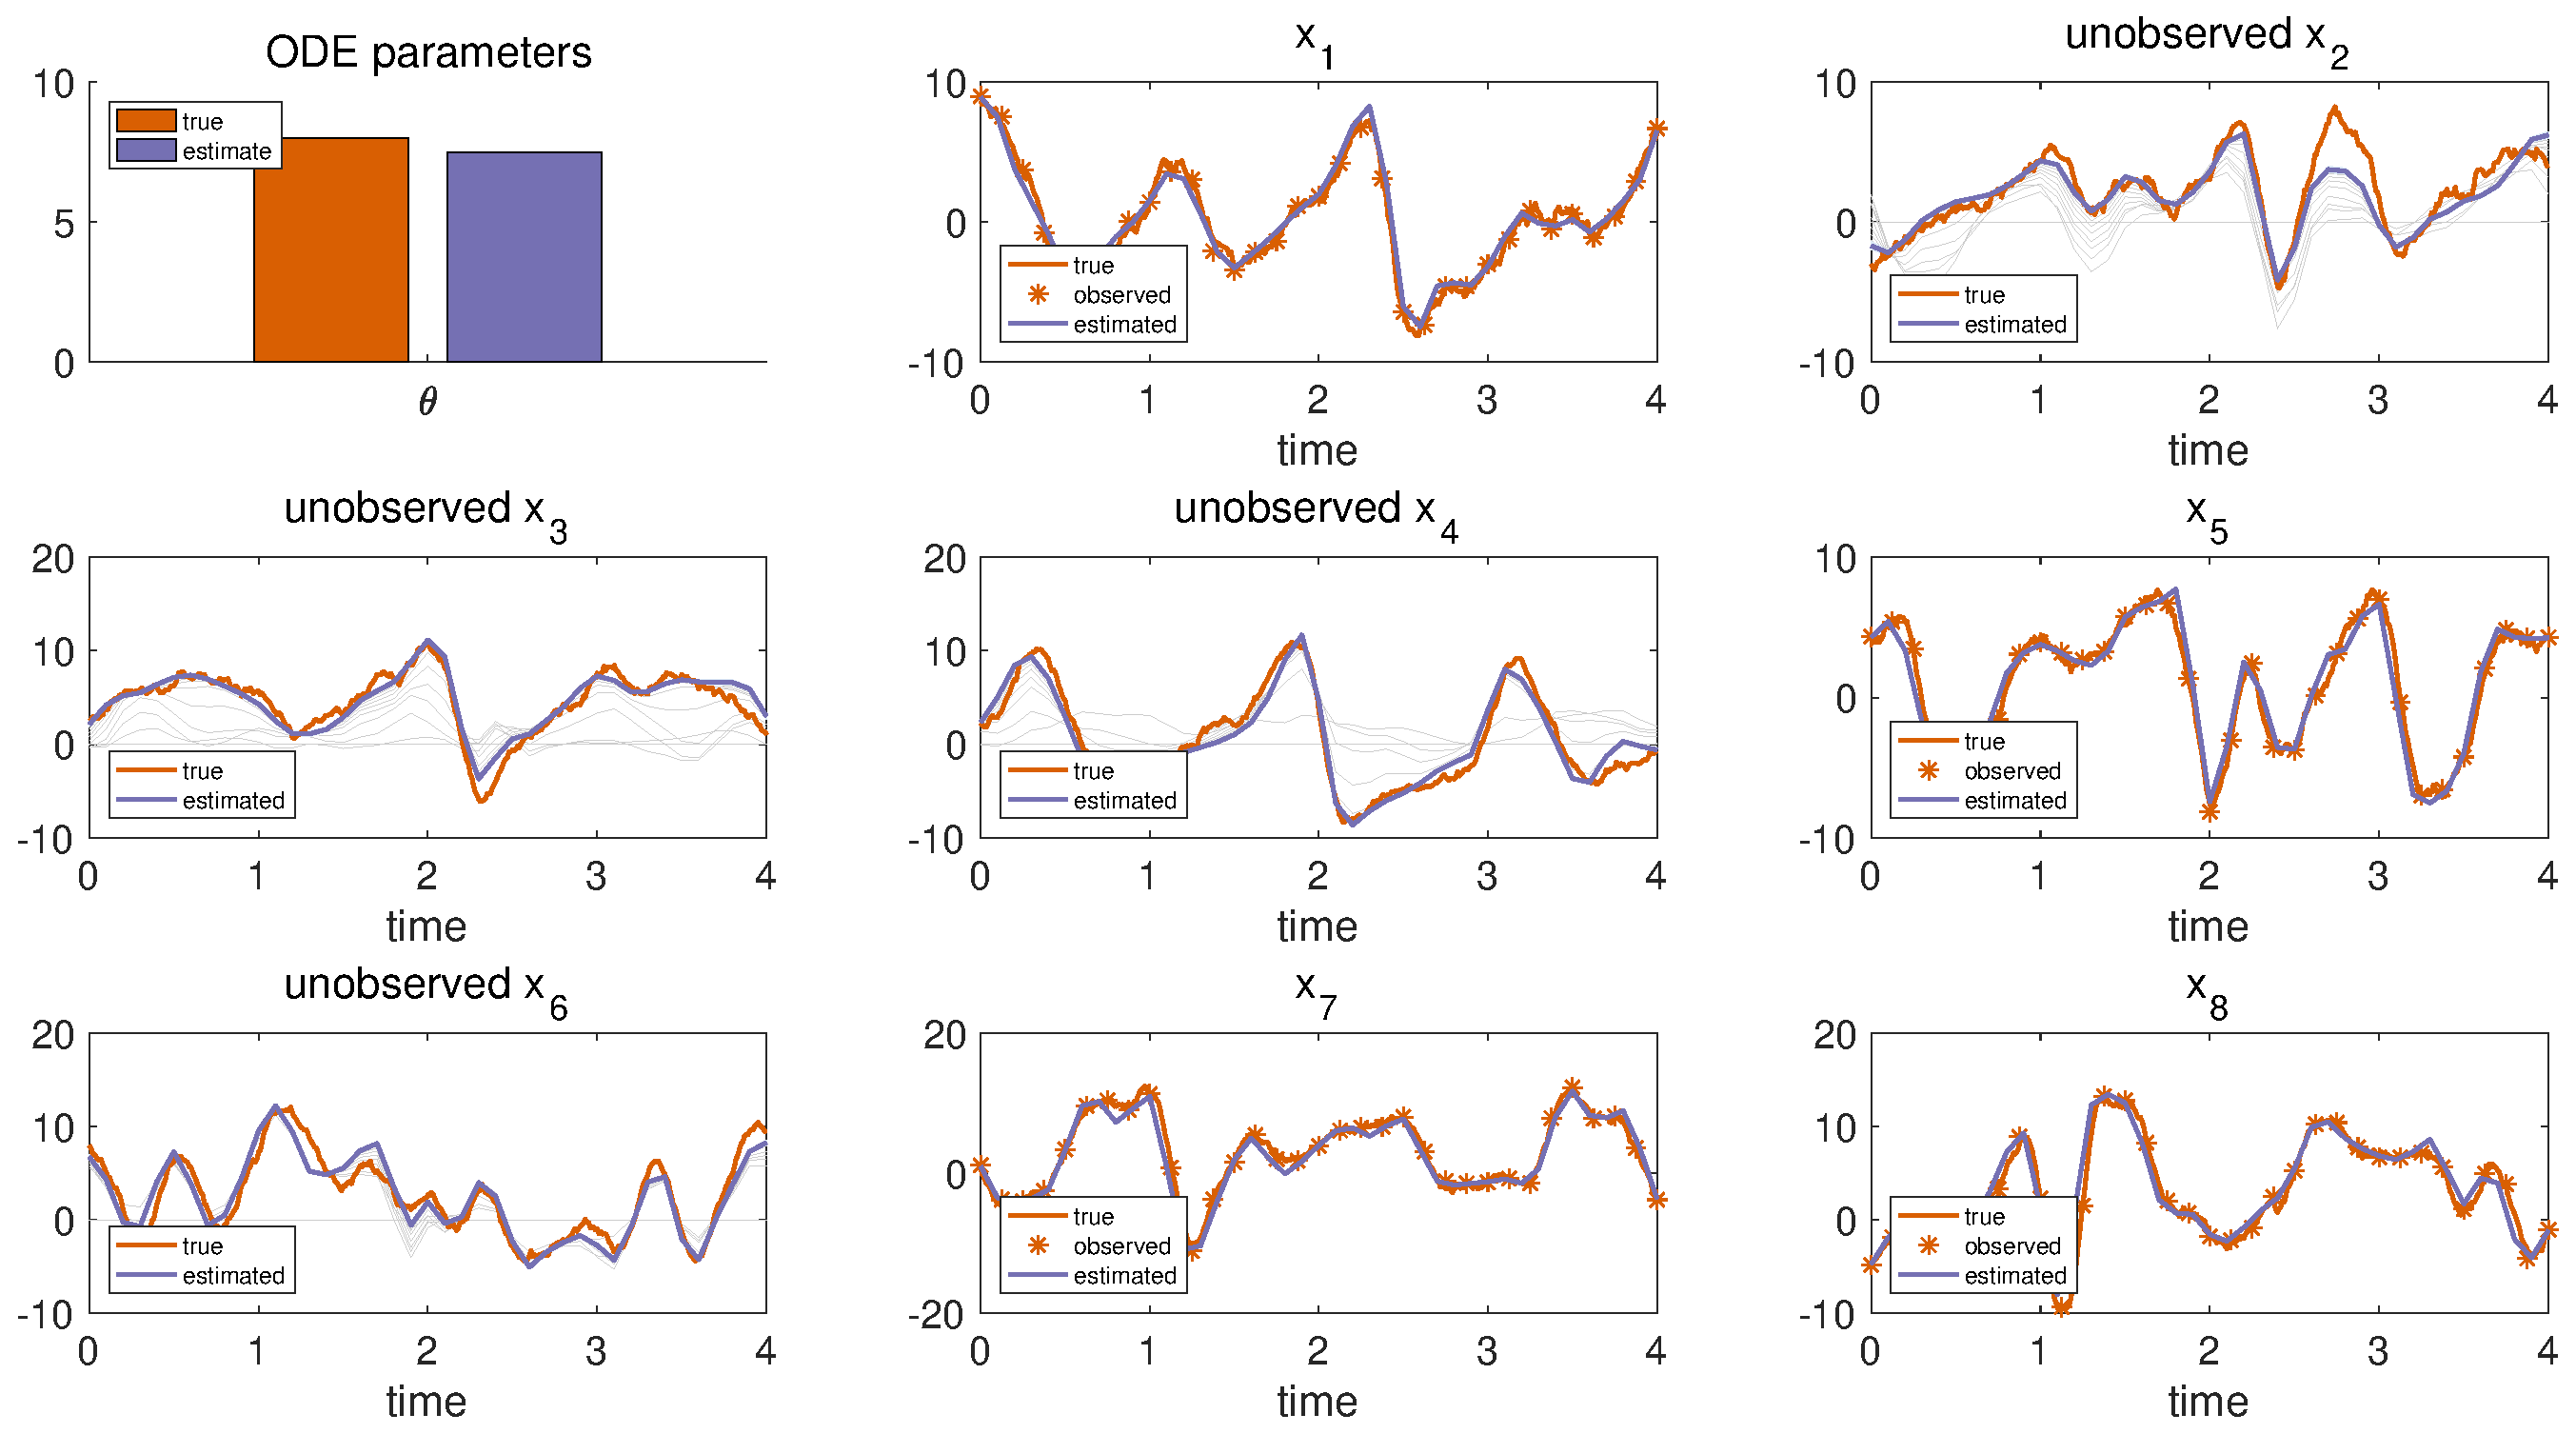
\includegraphics [width=5in]{Lorenz96_2_15.eps}
}

\section{Time Taken}

\color{RoyalPurple}\begin{verbatim}
disp(['time taken: ' num2str(toc) ' seconds'])
\end{verbatim}
\color{black}

        \begin{verbatim}time taken: 388.2428 seconds
\end{verbatim}
\color{black}
   